\documentclass{beamer}
 
\usepackage[utf8]{inputenc}

\usepackage{polyglossia}
\setdefaultlanguage{english}
\setotherlanguage{russian}

\usepackage{graphicx}
\setlength\fboxsep{3pt}
\setlength\fboxrule{1pt}

\usepackage{array,tabularx,tabulary,booktabs}
\usepackage{adjustbox} 

\usepackage{hyperref}

\usepackage{pythonhighlight}
\usepackage{listings}
\usepackage{lstautogobble}
\usepackage{color}
\usepackage{zi4}
\lstset{
    autogobble,
    columns=fullflexible,
    showtabs=false,
    breaklines=true,
    showstringspaces=false,
    breakatwhitespace=true,
    escapeinside={(*@}{@*)},
    tabsize=4,
}

\usepackage[autostyle]{csquotes}
\usepackage[backend=biber,style=authoryear]{biblatex}
\addbibresource{mybiblio.bib}
 
\title{Python Library for Linguistic Typology}
\author[Michael Voronov]{Michael Voronov\\{\small Scientific Advisor: Boris Orekhov}}
\institute{Higher School of Economics}
\date{18.06.2019}
 
\begin{document}
 
\frame{\titlepage}
 
\begin{frame}
\frametitle{Introduction}
Problem:
\begin{itemize}
 \item No Python tools for online linguistic databases queries.
 \item No Python tools for linguistic interactive mapping.
\end{itemize}
What exists?
\begin{itemize}
 \item R package \textbf{lingtypology} that does both \parencite{GeorgeMoroz2018}.
\end{itemize}
Why Python?
\begin{itemize}
 \item De-facto standard language among linguists.
 \item A lot of scientific libraries (Pandas, SciPy etc.)
 \item Unicode out of the box.
 \item Relatively high speed.
 \item Versatile language.
\end{itemize}
\end{frame}
 
\begin{frame}
\frametitle{Used Tools}
\begin{itemize}
 \item Python \parencite{python}
 \item Pandas \parencite{pandas}
 \item Folium \parencite{folium}
 \item Matplotlib \parencite{matplotlib}
 \item PyGlottolog \parencite{Robert2Forkel2019}
 \item SciPy \parencite{scipy}
\end{itemize}
\end{frame}


\begin{frame}
\frametitle{Project Description}
Remote Repository:
\begin{itemize}
 \item \url{https://github.com/OneAdder/lingtypology}
\end{itemize}
Documentation:
\begin{itemize}
 \item \url{https://oneadder.github.io/lingtypology/}
\end{itemize}
Modules:
\begin{itemize}
 \item \texttt{lingtypology.maps}
 \item \texttt{lingtypology.datasets}
 \item \texttt{lingtypology.glottolog}
\end{itemize}
\end{frame}

\begin{frame}[fragile]
\frametitle{Maps}
\begin{python}
languages = ('Romanian', 'Afrikaans', 'Tlingit', 'Japanese')
m = lingtypology.LingMap(languages)
m.create_map()
\end{python}
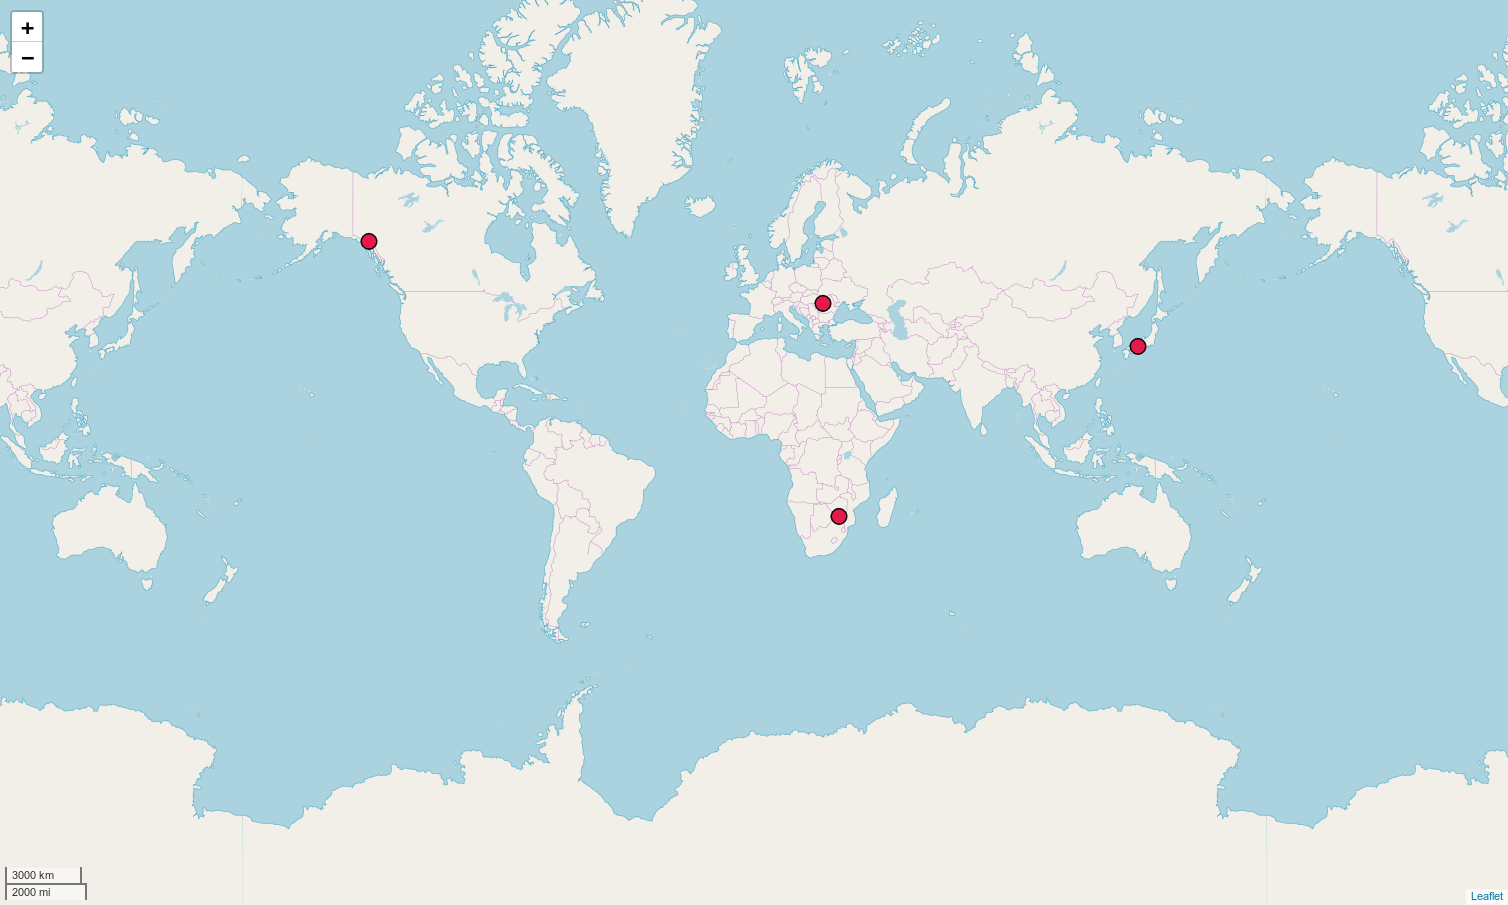
\includegraphics[width=\textwidth]{images/SimpleMap.png}
\end{frame}

\begin{frame}[fragile]
\frametitle{Maps}
\begin{python}
languages = [
    "Adyghe", "Kabardian", "Polish",
    "Russian", "Bulgarian"
]
features = [
    "Agglutinative", "Agglutinative", "Inflected",
    "Inflected", "Analytic"
]
m = lingtypology.LingMap(languages)
m.add_features(features)
m.create_map()
\end{python}
\end{frame}

\begin{frame}
\frametitle{Maps}
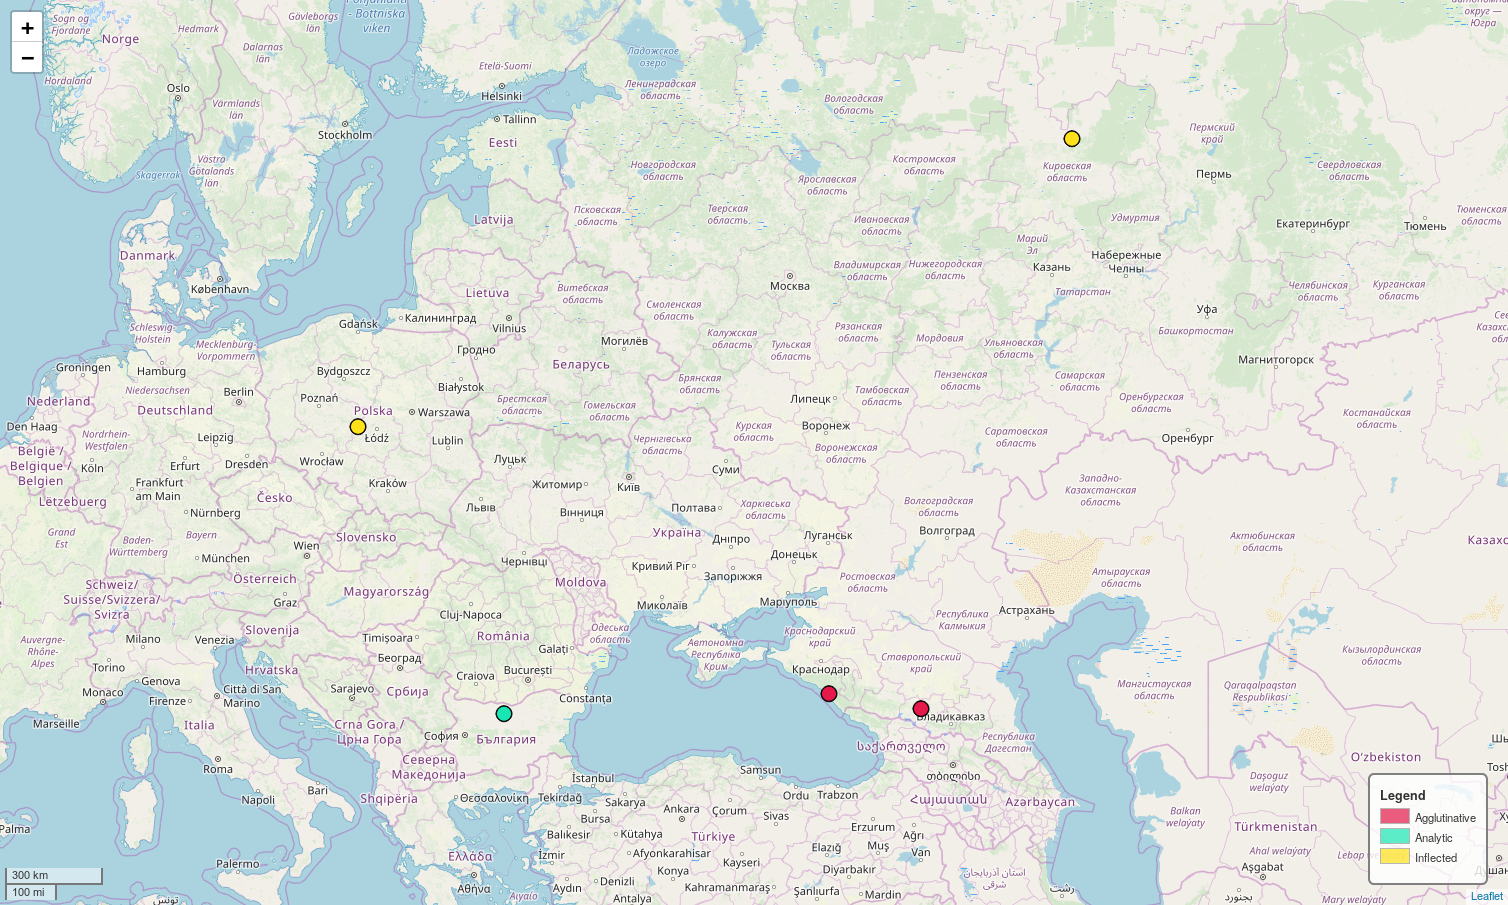
\includegraphics[width=\textwidth]{images/FeaturesMap.png}
\end{frame}

\begin{frame}[fragile]
\frametitle{Maps}
\begin{python}
m = lingtypology.LingMap(data.language)
m.add_minicharts(data.consonants, data.vowels)
m.create_map()
\end{python}
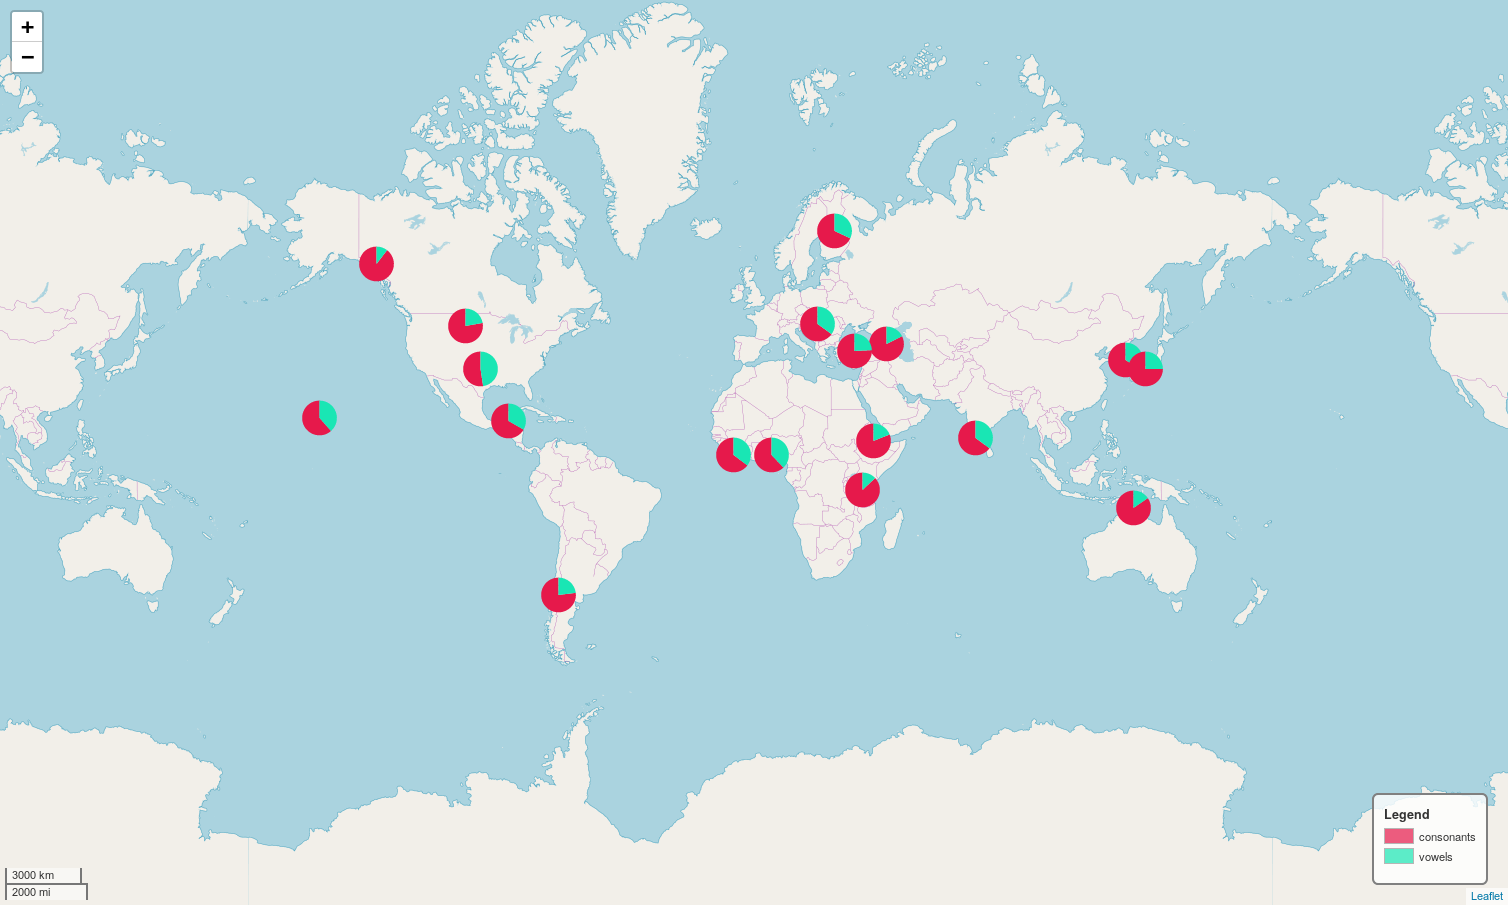
\includegraphics[width=\textwidth]{images/MinichartsMap.png}
\end{frame}

\begin{frame}
\frametitle{Databases}
\begin{itemize}
 \item WALS: The World Atlas of Language Structures \parencite{wals}.
 \item Autotyp: an international network of typological linguistic databases \parencite{autotyp}.
 \item AfBo: A world-wide survey of affix borrowing \parencite{afbo}.
 \item SAILS: The South American Indigenous Language Structures \parencite{sails}.
 \item PHOIBLE: ... is a repository of cross-linguistic phonological inventory data \parencite{phoible}.
\end{itemize}
\end{frame}

\begin{frame}[fragile]
\frametitle{WALS}
\begin{python}
w = lingtypology.datasets.Wals('1a')
w.get_df().head(10)
\end{python}
\begin{adjustbox}{max width=\textwidth}
\begin{tabular}{llllllllrl}
\toprule
{} & wals\_code &           language &                genus &               family &                      coordinates &   \_1A\_area &                  \_1A &  \_1A\_num &          \_1A\_desc \\
\midrule
0 &       kiw &   Kiwai (Southern) &              Kiwaian &              Kiwaian &                    (-8.0, 143.5) &  Phonology &             1. Small &        1 &             Small \\
1 &       xoo &               !Xóõ &                   Tu &                   Tu &                    (-24.0, 21.5) &  Phonology &             5. Large &        5 &             Large \\
2 &       ani &              //Ani &           Khoe-Kwadi &           Khoe-Kwadi &  (-18.9166666667, 21.9166666667) &  Phonology &             5. Large &        5 &             Large \\
3 &       abi &             Abipón &     South Guaicuruan &           Guaicuruan &                   (-29.0, -61.0) &  Phonology &  2. Moderately small &        2 &  Moderately small \\
4 &       abk &             Abkhaz &  Northwest Caucasian &  Northwest Caucasian &            (43.0833333333, 41.0) &  Phonology &             5. Large &        5 &             Large \\
5 &       acm &           Achumawi &          Palaihnihan &                Hokan &                   (41.5, -121.0) &  Phonology &  2. Moderately small &        2 &  Moderately small \\
6 &       ach &               Aché &         Tupi-Guaraní &               Tupian &         (-25.25, -55.1666666667) &  Phonology &             1. Small &        1 &             Small \\
7 &       aco &              Acoma &              Keresan &              Keresan &  (34.9166666667, -107.583333333) &  Phonology &             5. Large &        5 &             Large \\
8 &       adz &             Adzera &              Oceanic &         Austronesian &                  (-6.25, 146.25) &  Phonology &  2. Moderately small &        2 &  Moderately small \\
9 &       agh &              Aghem &              Bantoid &          Niger-Congo &        (6.666666666669999, 10.0) &  Phonology &           3. Average &        3 &           Average \\
\bottomrule
\end{tabular}
\end{adjustbox}
\end{frame}

\begin{frame}[fragile]
\frametitle{WALS}
\begin{python}
w = lingtypology.datasets.Wals('1a', '2a')
w.get_df().head()
\end{python}
\begin{adjustbox}{max width=\textwidth}
\begin{tabular}{llclclc}
\toprule
{} &           language & ... & \_1A & ... & \_2A & ... \\
\midrule
0 &   Kiwai (Southern) & ... &  1. Small & ... &  2. Average (5-6) & ...\\
1 &               !Xóõ & ... &  5. Large & ... &  2. Average (5-6) & ...\\
2 &              //Ani & ... &  5. Large & ... &  2. Average (5-6) & ...\\
3 &             Abipón & ... &  2. Moderately small & ... &  2. Average (5-6) & ...\\
4 &             Abkhaz & ... &  5. Large & ... &    1. Small (2-4) & ...\\
\bottomrule
\end{tabular}
\end{adjustbox}
\end{frame}

\begin{frame}[fragile]
\frametitle{Examples: WALS Features}
\begin{python}
wals_page = lingtypology.datasets.Wals('1a').get_df()
m = lingtypology.LingMap(wals_page.language)
m.add_custom_coordinates(wals_page.coordinates)
m.add_features(
    wals_page._1A,
    colors=lingtypology.gradient(5, 'yellow', 'green')
)
m.legend_title = 'Consonant Inventory'
m.create_map()
\end{python}
\end{frame}

\begin{frame}
\frametitle{Examples: WALS Features}
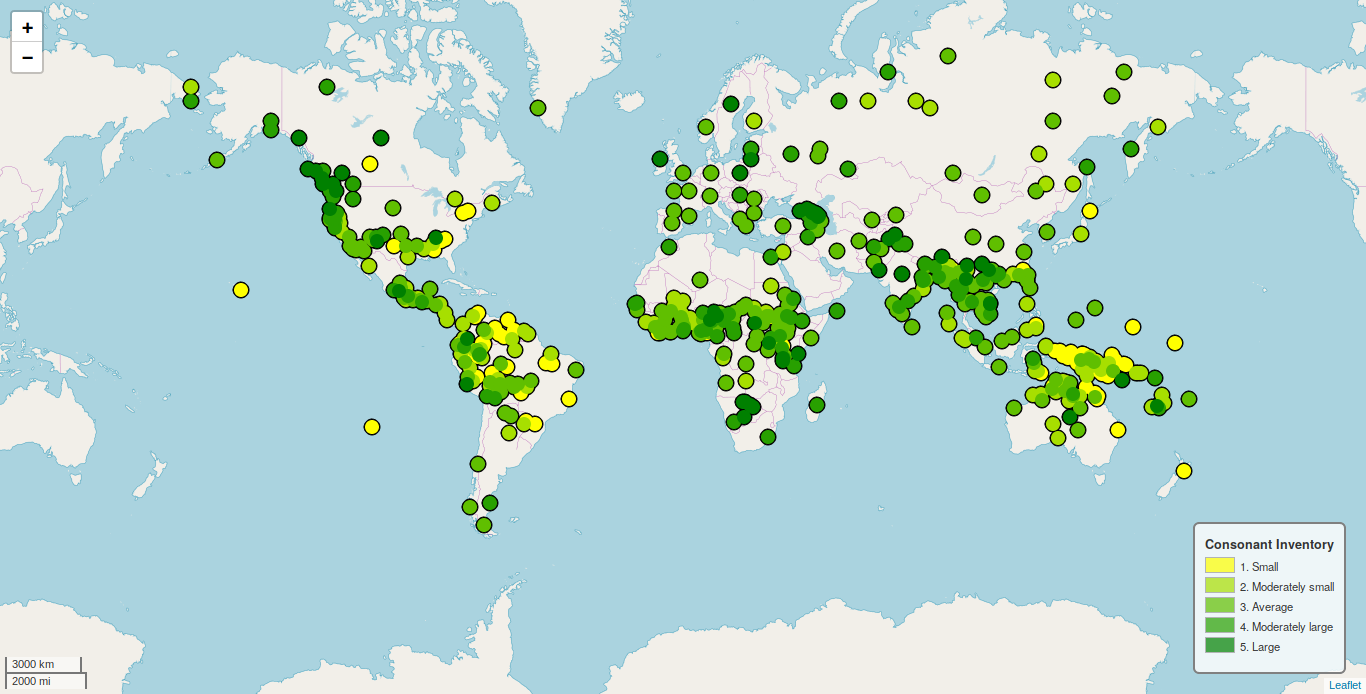
\includegraphics[width=\textwidth]{images/LingtypologyStrokeAppearance.png}
\end{frame}

\begin{frame}[fragile]
\frametitle{Examples: WALS Heatmap}
\begin{python}
wals = lingtypology.datasets.Wals('1A')
data = wals.get_df()
m = lingtypology.LingMap()
m. add_heatmap(data[data._1A_desc == 'Large'].coordinates)
m.create_map()
\end{python}
\end{frame}

\begin{frame}
\frametitle{Examples: WALS Heatmap}
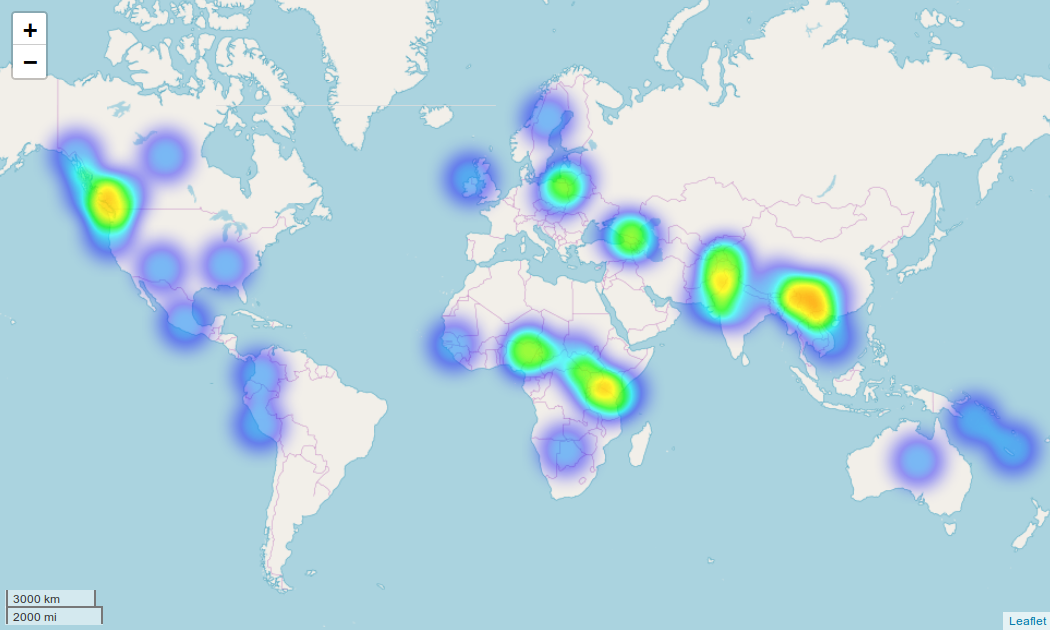
\includegraphics[width=\textwidth]{images/WalsHeatMap2.png}
\end{frame}

\begin{frame}[fragile]
\frametitle{Examples: PHOIBLE Tones}
\begin{python}
p = lingtypology.datasets.Phoible(subset='SPA')
df = p.get_df(strip_na=['tones'])
m = lingtypology.LingMap(df.language)
m.add_features(df.tones, numeric=True)
m.colormap_colors = ('white', 'red')
m.legend_title = 'Tones'
m.legend_position = 'bottomleft'
m.create_map()
\end{python}
\end{frame}

\begin{frame}
\frametitle{Examples: PHOIBLE Tones}
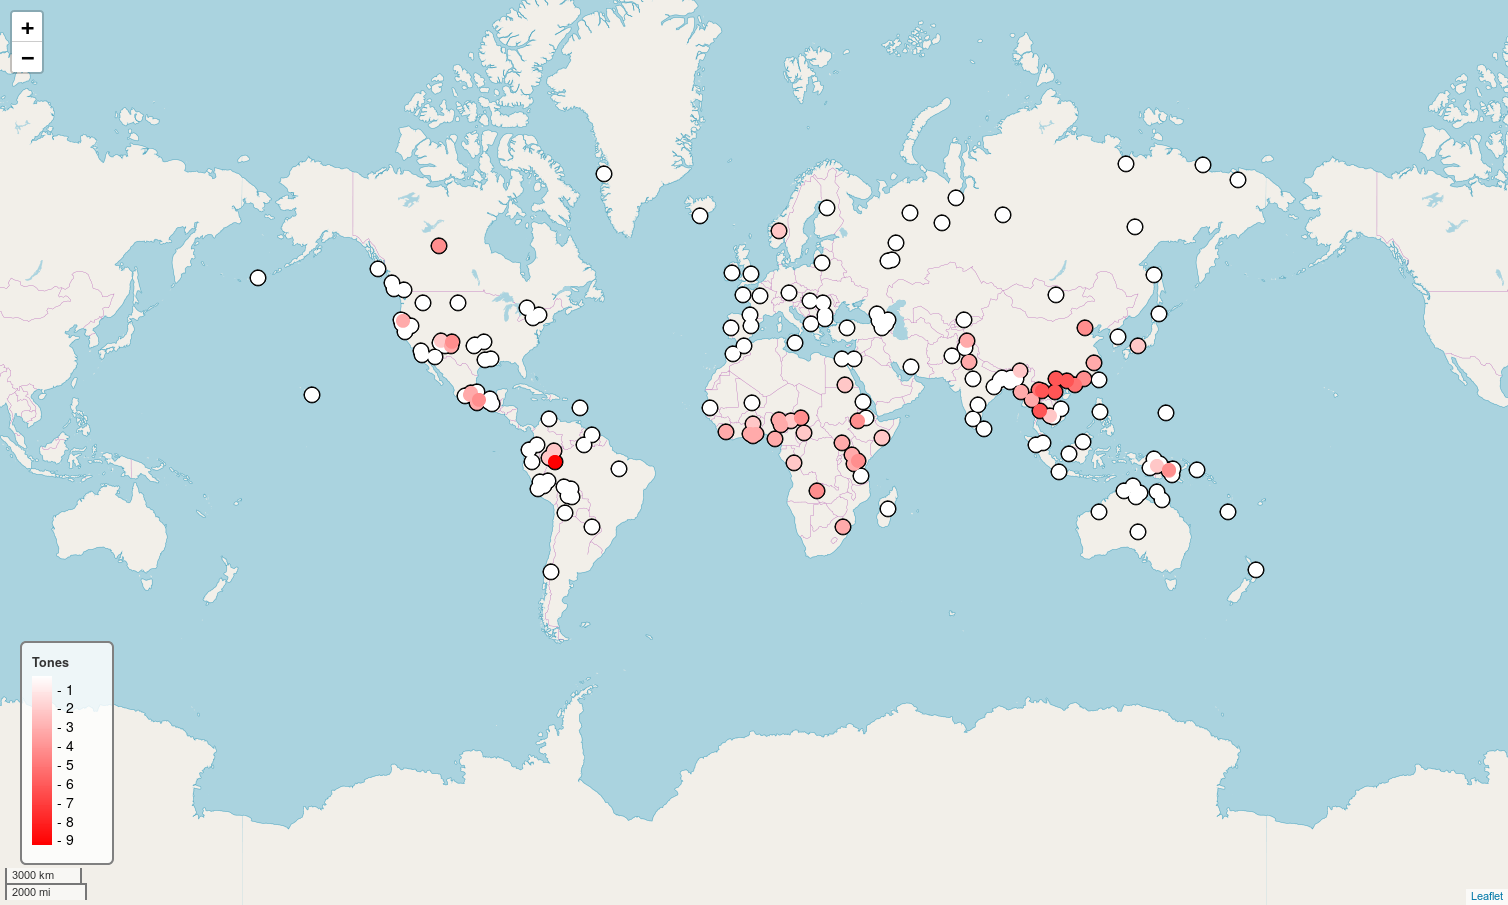
\includegraphics[width=\textwidth]{images/PHOIBLE.png}
\end{frame}

\begin{frame}
\frametitle{Verification of Statistical Studies in the Context of Reproducibility}
\begin{itemize}
 \item Article that demonstrates relationship between presence of ejectives and high elevation based on WALS data \parencite{ejectives}.
 \item Reproduce on PHOIBLE data.
\end{itemize}
\end{frame}

\begin{frame}[fragile]
\frametitle{Verification of Statistical Studies in the Context of Reproducibility}
\begin{python}
upsid = lingtypology.datasets.Phoible(
    subset='UPSID',
    aggregated=False
).get_df()
amount_of_ejectives = upsid[
    upsid.raisedLarynxEjective == '+'
].groupby('Glottocode').size()
languages = [
    lingtypology.glottolog.get_by_glot_id(glot_id) \
    for glot_id in amount_of_ejectives.index
]
upsid_ejectives = pandas.DataFrame({
    'language': languages,
    'ejectives': amount_of_ejectives,
    'elevation': lingtypology.get_elevations(languages),
})
m = lingtypology.LingMap(upsid_ejectives.language)
m.add_features(upsid_ejectives.elevation, numeric=True)
m.create_map()
\end{python}
\end{frame}

\begin{frame}
\frametitle{Verification of Statistical Studies in the Context of Reproducibility}
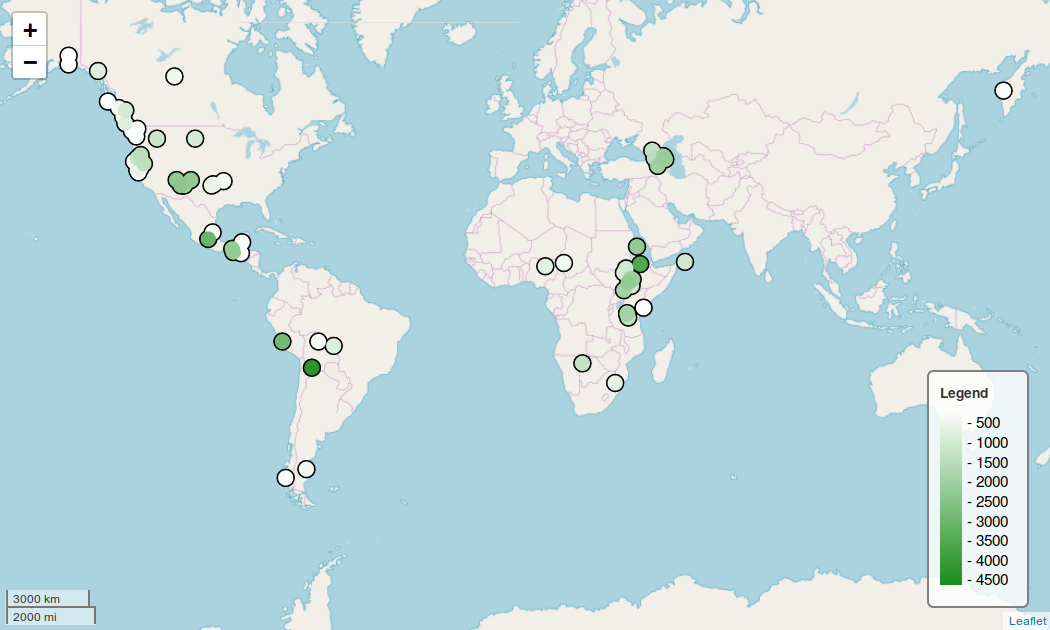
\includegraphics[width=\textwidth]{images/EjectivesElevation.png}
\end{frame}

\begin{frame}
\frametitle{Verification of Statistical Studies in the Context of Reproducibility}
PHOIBLE datasets:
\begin{itemize}
 \item SAPHON: South American Phonological Inventory Database~\parencite{saphon}.
 \item AA: Alphabets of Africa~\parencite{aa}.
 \item GM: `Christopher Green and Steven Moran extracted phonological inventories from secondary sources including grammars and phonological descriptions with the goal of attaining pan-Africa coverage`~\parencite{gm}.
\end{itemize}
\end{frame}

\begin{frame}
\frametitle{Verification of Statistical Studies in the Context of Reproducibility}
\begin{itemize}
 \item PH: `Christopher Green and Steven Moran extracted phonological inventories from secondary sources including grammars and phonological descriptions with the goal of attaining pan-Africa coverage`~\parencite{gm}.
 \item RA: Common Linguistic Features in Indian Languages: Phoentics~\parencite{ra}.
 \item SPA: Stanford Phonology Archive~\parencite{spa}.
 \item UPSID: UCLA Phonological Segment Inventory Database~\parencite{upsid}.
\end{itemize}
\end{frame}

\begin{frame}
\frametitle{Verification of Statistical Studies in the Context of Reproducibility}
\begin{adjustbox}{max width=\textwidth}
\begin{tabular}{l|l|ccc}
    \toprule
    ~  & Dataset  & Regression (with ejectives only)  & Regression (all languages)  & Chi2 Test \\
    \midrule
    0  & UPSID  & 0.95055  & 0.00004  & 0.00003 \\
    1  & SPA  & 0.47553  & 0.00001  & 0.00018 \\
    2  & PH  & 0.73152  & 0.39245  & 0.16019 \\
    3  & GM  & 0.03858  & 0.00000  & 0.00000 \\
    4  & SAPHON  & 0.018874  & 0.00000  & 0.00038 \\
    \bottomrule
\end{tabular}
\end{adjustbox}
\end{frame}

\begin{frame}
\frametitle{Verification of Statistical Studies in the Context of Reproducibility}
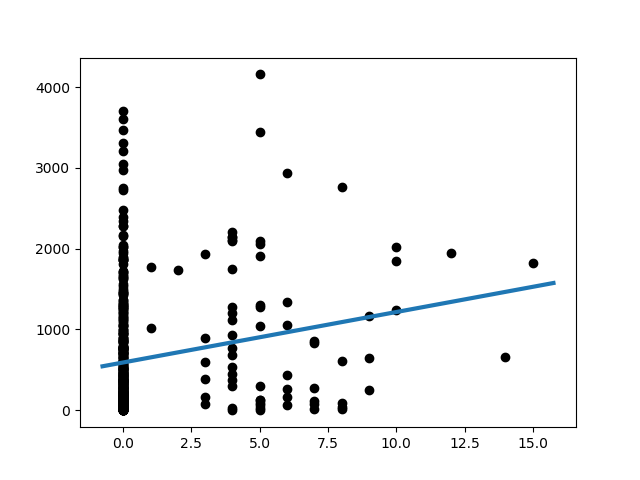
\includegraphics[width=\textwidth]{images/linear_regression_raisedLarynxEjective_all.png}
\end{frame}

\begin{frame}
\frametitle{Verification of Statistical Studies in the Context of Reproducibility}
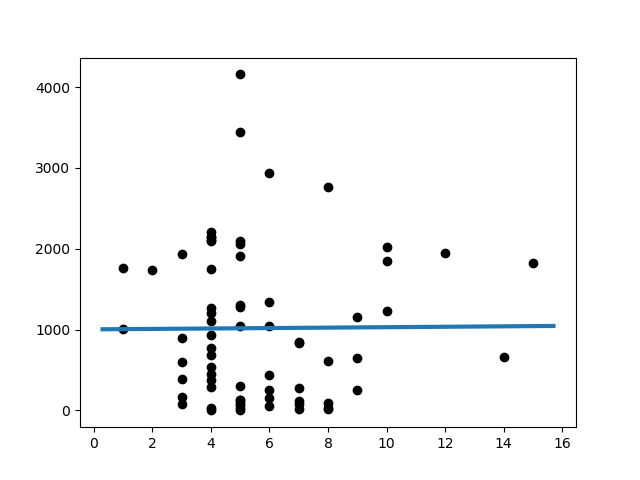
\includegraphics[width=\textwidth]{images/linear_regression_raisedLarynxEjective_only.png}
\end{frame}

\begin{frame}
\frametitle{Verification of Statistical Studies in the Context of Reproducibility}
Results:
\begin{itemize}
 \item True: share of languages with ejectives is higher if the elevation is more than 1500m (verified on PHOIBLE data).
 \item Not true: the higher the language, the more ejectives there are.
\end{itemize}
\end{frame}

\begin{frame}
\frametitle{PHOIBLE and Elevation}
\begin{tabular}{llcccc}
\toprule
{} & Dataset &     short &      long & delayedRelease & ... \\
\midrule
0 &   UPSID &    0.7304 &    0.6205 &         0.6106 &    ... \\
1 &     SPA &    0.4974 &    0.8311 &         0.4335 &    ... \\
2 &      GM &    0.6587 &    0.0070 &         0.8435 &    ... \\
3 &      RA &    0.0826 &    0.1125 &            nan &    ... \\
5 &      AA &       NaN &    0.7559 &            nan &    ... \\
6 &      PH &       NaN &    0.2549 &         0.9051 &    ... \\
7 &  SAPHON &       NaN &    0.0287 &         0.4856 &    ... \\
\midrule
4 &  Median &  0.578074 &  0.254949 &       0.610642 &    ... \\
\bottomrule
\end{tabular}

Full Table: \url{https://github.com/OneAdder/lingtypology_research/blob/master/PHOIBLE:\%20Quantitative\%20Research.ipynb}
\end{frame}

\begin{frame}
\frametitle{Autotyp and Elevation}
\begin{itemize}
 \item `Exponence: number of categories that are expressed in the same marker`.
 \item `Rough approximation of the size of the possessum category in terms of the number of semantic classes covered`.
 \item `Number of separately marked inflectional categories (including agreement) in position "post" of the verb`.
 \item `Number of morpheme types included in a phonologically or grammatically coherent suffix domain`.
\end{itemize}
\end{frame}

\begin{frame}
\frametitle{Autotyp and Elevation}
\begin{adjustbox}{max width=\textwidth}
\begin{tabular}{lll}
\toprule
Feature &                    Subfeature &     P-value \\
\midrule
Grammatical\_markers &                   Exponence.n &  0.00000000 \\
NP\_structure &          NPHeadSemClassSize.n &  0.01766784 \\
VInfl\_counts\_per\_position &          VInflCatAndAgrPost.n &  0.02895302 \\
Word\_domains &  MphmTypesInCohSuffixDomain.n &  0.00196901 \\
\bottomrule
\end{tabular}
\end{adjustbox}
\end{frame}

\begin{frame}
 \frametitle{Autotyp and Elevation}
 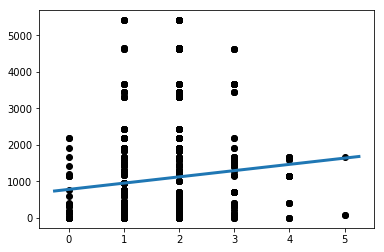
\includegraphics[width=\textwidth]{images/AutotypRegr.png}
\end{frame}

\begin{frame}
\frametitle{WALS: Implicative Universaliae}
\begin{adjustbox}{max width=\textwidth}
\begin{tabular}{|l|cccc|l|}
\hline
feature & \_10A\_desc & \_25B\_desc & \_39B\_desc & \_47A\_desc & ... \\
\hline
\_10A\_desc &   1.00000 &   0.99444 &       nan &   0.63296 &   ... \\
\_25B\_desc &   0.90442 &   1.00000 &       nan &   0.96609 &   ... \\
\_39B\_desc &   1.00000 &       nan &   1.00000 &   0.66501 &   ... \\
\_47A\_desc &   0.82120 &   0.84267 &   0.66501 &   1.00000 &   ... \\
\hline
... &   ... &   ... &       ... &   ... &   ... \\
\hline
\end{tabular}
\end{adjustbox}
Full table: \url{https://github.com/OneAdder/lingtypology_research/blob/master/WALS:\%20Quantitative\%20Research.ipynb}
\end{frame}

\begin{frame}
\frametitle{Conclusion}
\begin{itemize}
 \item LingTypology: a Python tool for linguistic typology
 \begin{itemize}
  \item Repository: \url{https://github.com/OneAdder/lingtypology}
  \item Documentation: \url{https://oneadder.github.io/lingtypology/}
  \item PyPI: \url{https://pypi.org/project/lingtypology/}
 \end{itemize}
 \item Demonstrative Studies
 \begin{itemize}
  \item Simplicity
  \item Reproducibility
  \item Visualization
 \end{itemize}
\end{itemize}

\end{frame}

\begin{frame}[allowframebreaks]
\frametitle{References}
\renewcommand*{\bibfont}{\tiny}
\printbibliography
\end{frame}

\end{document}
